% Chapter 1

\chapter{Introducción general} % Main chapter title

\label{Chapter1} % For referencing the chapter elsewhere, use \ref{Chapter1}
\label{IntroGeneral}

%----------------------------------------------------------------------------------------

% Define some commands to keep the formatting separated from the content
\newcommand{\keyword}[1]{\textbf{#1}}
\newcommand{\tabhead}[1]{\textbf{#1}}
\newcommand{\code}[1]{\texttt{#1}}
\newcommand{\file}[1]{\texttt{\bfseries#1}}
\newcommand{\option}[1]{\texttt{\itshape#1}}
\newcommand{\grados}{$^{\circ}$}

%----------------------------------------------------------------------------------------

%\section{Introducción}
%citas \citep{ARTICLE:1}
%----------------------------------------------------------------------------------------
%s
En el presente capítulo se describe el funcionamiento de un sistema de detección de incendio convencional, la lógica que suelen tener los protocolos de notificación de eventos, y las tecnologías actuales de monitoreo remoto que existen. Finalmente se detallan los motivos del proyecto enfocado a las necesidades del mercado argentino. 


\section{Sistemas de alarma de incendio.}
%
La detección de incendios es una herramienta preventiva clave para la seguridad humana \citep{rev_innov_1}, a su vez corresponde a un elemento de vital importancia para la evacuación exitosa ante situaciones de emergencia. En diferentes ciudades del mundo son considerados requisitos indispensables para poder categorizar a un establecimiento como habitable.

A partir del código de edificación dispuesto desde el año 2019 en la Ciudad de Buenos Aires \citep{cod_edif}, se establece que los sistemas de detección de alarma de incendio (SDAI) son requisitos obligatorios para diferentes tipos de recintos. A su vez, se debe considerar que contar con un SDAI no significa que el recinto se encuentre debidamente protegido, esto se evidencia en la Ley 5920 \citep{ley_5920}. En la que se exige a los establecimientos presentar un sistema de autoprotección \citep{rev_innov_2}, en el cual se incluye entre sus elementos obligatorios un plan de evacuación y la designación de personas con un rol específico, en el caso de requerir ejecutar procedimientos de emergencia. En otras palabras, a pesar de que efectivamente un SDAI es un elemento invaluable para una edificación, desde un punto de vista legal por sí mismo no es suficiente como única medida de protección. 

Los protocolos de evacuación usualmente se apoyan en sistemas automatizados y especifican la serie de acciones, modos, pautas y tiempos estimados de evacuación. Los beneficios más significativos de contar con un SDAI se pueden reducir en tres principales: evitar la inhalación de humo, detección temprana y monitoreo ininterrumpido. El beneficio primordial es la detección temprana, ya que minimiza el tiempo de reacción de los ocupantes y en conjunto con un sistema de notificación eficiente, pueden dar inicio a la toma de acciones por parte del personal especializado, lo que disminuye el tiempo total de evacuación. \citep{utn_1}\citep{plan_evac}.
\subsection{Sistemas de detección de alarma de incendio convencionales}
%

En la figura \ref{fig:sdai_conv} podemos observar la distribución de un SDAI básico, es evidente que los sistemas de detección de incendio cuentan con dos componentes clave, con un objetivo específico:
\begin{itemize}
\item Circuito de detección: circuito eléctrico que comprende aquellos dispositivos cuya finalidad es detectar (mediante el monitoreo de fenómenos físicos) los focos de incendio. Por ejemplo: detectores de humo, iónicos, llama, avisadores manuales, etc.
\item Circuito de notificación: a diferencia del circuito de detección, estos dispositivos reaccionan una vez detectado el foco de incendio. La función de estos dispositivos es dar aviso a los ocupantes del recinto en caso de una alarma de incendio. Por ejemplo: sirenas, luces estroboscópicas, sistemas de audio, accionamiento de contactos eléctricos, etc.
\end{itemize}
\begin{figure}[ht]
    \centering
    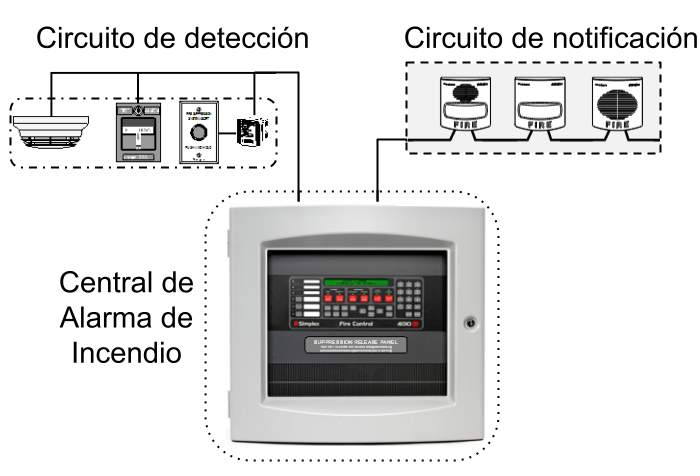
\includegraphics[scale=.45]{./Figures/sdai_conv.png}
    \caption{Esquema de un SDAI básico.}
    \label{fig:sdai_conv}
\end{figure}

Por lo general una central de alarma de incendio (CAI) realiza las tareas de monitorear, registrar, notificar y finalmente reaccionar a eventos de falla y/o alarma en la instalación. Todos los eventos cuentan con notificación visual y sonora en la CAI, sin embargo el accionamiento del circuito de notificación depende del protocolo de evacuación implementado. La figura \ref{fig:flujo_conv} aclara el flujo de procesamiento usual de un evento de alarma, primero la etapa de detección, luego reporte en en la CAI con los datos del dispositivo y finalmente una etapa de notificación a los usuario según el protocolo de evacuación.

\begin{figure}[ht]
    \centering
    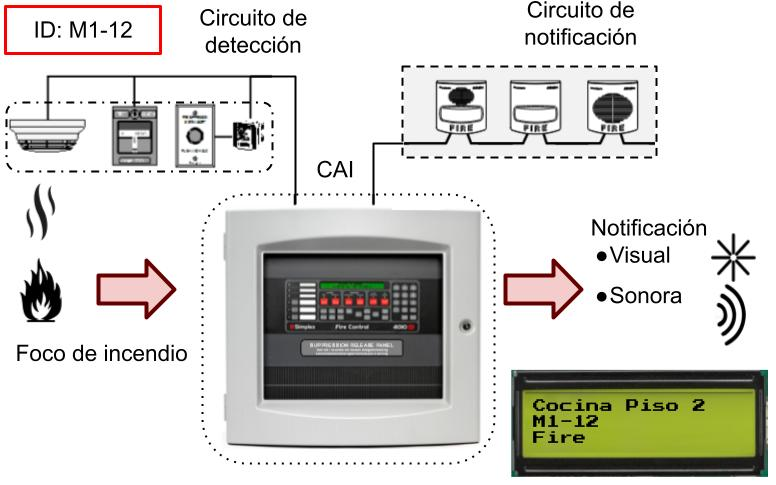
\includegraphics[scale=.45]{./Figures/flujo_conv.jpg}
    \caption{Flujo en caso de un evento de alarma.}
    \label{fig:flujo_conv}
\end{figure}


\subsection{Sistemas de detección de alarma de incendio propuesto}
%
La estructura descrita en la figura \ref{fig:sdai_conv} comprende un SDAI básico, cuenta con lo mínimo requerido para establecer un esquema de protección. Generalmente para instalaciones pequeñas estos servicios suelen ser suficientes, pero existen factores que incrementan las exigencias de protección como por ejemplo: grandes superficies a proteger, múltiples zonas de riesgo en una misma instalación, zonas con diferentes niveles de propagación de incendio, etc. Estos factores hacen necesario que los fabricantes diseñen equipos con la posibilidad de expandir su rango de trabajo e incluso incluir nuevas funcionalidades.

Uno de los factores clave en el diseño de una CAI es la usabilidad, el sistema debe indicar de forma simple y eficiente la aparición de un evento. Esta interfaz debe ser clara con respecto a la información proveniente de un dispositivo de detección, pero también debe permitir al usuario ejecutar comandos de manera rápida según el procedimiento de evacuación. No obstante, los SDAI se rigen por un marco normativo \citep{nfpa_1}, que a pesar de tener diferentes beneficios (como la estandarización de los procesos), a la vez requiere que el usuario conozca la terminología y procedimientos utilizados por la NFPA (National Fire Protection Association) \citep{nfpa_2}. 

Las normas y leyes vigentes exigen capacitaciones regulares con respecto al uso de los SDAI, sin embargo existen algunos factores como: el idioma, error humano, horarios de trabajo, rotación de personal, entre otras.  Que hacen muy improbable que una persona correctamente capacitada se encuentre presente en el la instalación al momento de que ocurra un evento. En la figura \ref{fig:flujo_conv_user} se puede observar el flujo de acciones que debería realizar una persona correctamente capacitada.

\begin{figure}[ht]
    \centering
    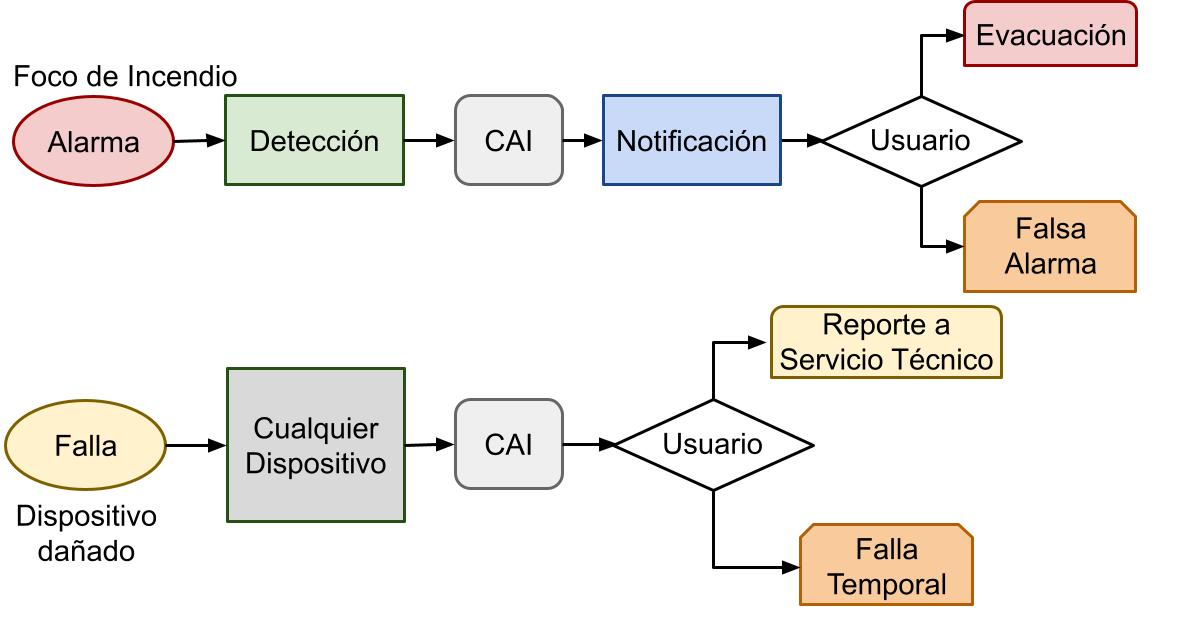
\includegraphics[scale=.3]{./Figures/flujo_dec.jpg}
    \caption{Flujo recomendado para el usuario en caso de eventos.}
    \label{fig:flujo_conv_user}
\end{figure}

Como se puede apreciar en la figura \ref{fig:flujo_conv_user}, el individuo es un elemento indispensable dentro del protocolo de evacuación. El SDAI puede de forma automática detectar y avisar ante focos de incendio, sin embargo las decisiones que se toman en esos primeros minutos afectan directamente el tiempo de reacción, cualquier error, confusión o inclusive inacción por parte del operario puede obstaculizar el éxito de la evacuación \citep{plan_evac}.

La figura \ref{fig:flujo_prop} representa al sistema propuesto, la diferencia radica en que se incluye un módulo de comunicación adicional, que establece conectividad con un servicio alocado en la nube. De esta forma es posible reportar de manera remota cualquier evento presente en el SDAI, no solo a las personas dentro de la instalación que puedan atender a las notificaciones de la central, sino también aquellas personas que interpretan un rol clave al momento de emergencias que puedan no estar al tanto de la situación. Por otro lado, en caso de producirse fallas en cualquiera de los circuitos antes mencionados, la notificación remota puede incluir al personal de mantenimiento. 

\begin{figure}[ht]
    \centering
    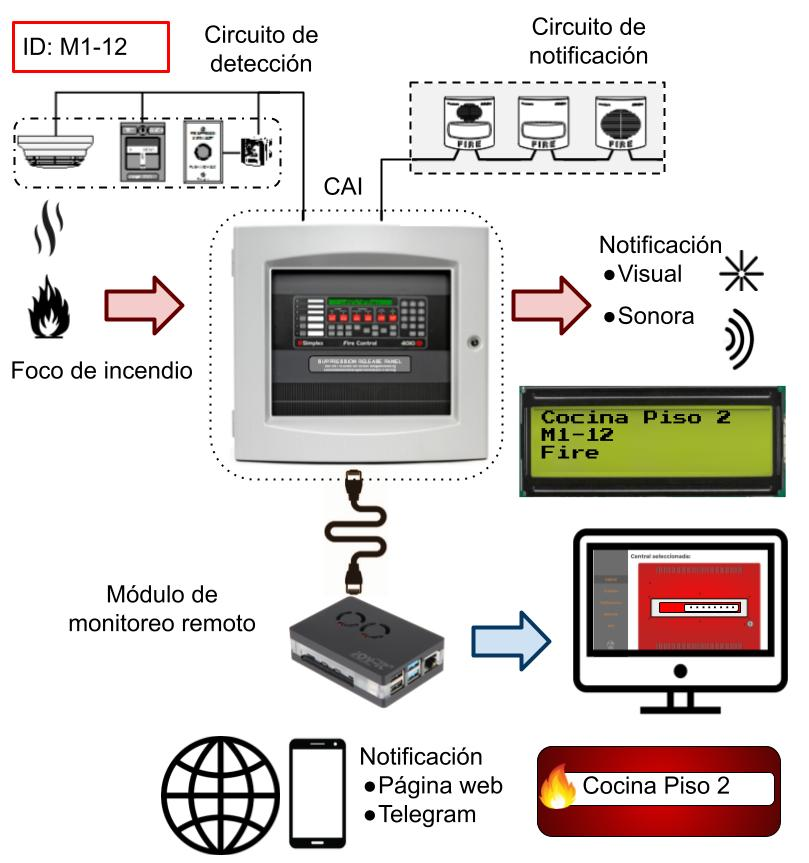
\includegraphics[scale=.45]{./Figures/flujo_prop.jpg}
    \caption{Flujo en caso de un evento de alarma, para el sistema propuesto.}
    \label{fig:flujo_prop}
\end{figure}

\section{Estado del arte}
%

En la tabla \ref{tab:comp} se comparan algunas de las alternativas comerciales. Todas las opciones se enfocan en incrementar el alcance de las notificaciones, sin embargo difieren según la marca del fabricante.

Por lo general cada fabricante cuenta con un protocolo de comunicación que permite a la CAI interactuar con el mundo exterior. Este protocolo suele ser RS232 o en algunos casos Telnet, sin embargo el formato de la información varía entre fabricantes. Es por esto que los sistemas de monitoreo remoto multi-plataforma suelen sacrificar la cantidad de información disponible de los eventos, de lo contrario se verían en la obligación de generar un esquema de decodificación por cada fabricante o incluso en algunos casos por cada modelo (como en el ítem 4 de la tabla \ref{tab:comp}). Desde otro punto de vista, si se incluye menor detalle por cada evento, es posible desarrollar un esquema multiplataforma que recolecte la información y la plasme sin necesidad de segmentarla (similar al ítem 1 de la tabla \ref{tab:comp}).

En un trabajo de investigación previo se desarrolló un sistema de monitoreo de CAI generales, este sistema permite conocer a un nivel básico el estado del SDAI (estado de alarma, falla o normal). El trabajo actual se enfoca en ampliar la cantidad de información que se presenta actualmente en la plataforma de monitoreo, un nivel completo de notificación incluye específicamente los siguientes detalles por dispositivo en caso de presentarse una anomalía o alarma: código, etiqueta, tipo y estado.



\begin{table}[h]
\centering
\caption[caption corto]{Comparación entre equipos comerciales actuales.}
\begin{tabular}{l c c c c c}
\toprule
\textbf{Nombre} & \textbf{Compatibilidad}& \textbf{Nivel de detalle}& \textbf{Ref}\\
\midrule
SNAI (CESE) & Múltiple & Básico & \citep{cese} \\
Safelinc & Simplex & Completo & \citep{safelinc} \\
HT-7001 & Múltiple & Básico & \citep{ht7001}\\
ONYXWORKS & Notifier & Completo & \citep{onyxworks}\\
Control Room Monitor & Múltiple & Completo & \citep{nimbus} \\
Security Server & Bosch & Completo & \citep{ss_bosch} \\
Fire Alarm Monitoring & Múltiple & Básico & \citep{churches}\\
Discador telefónico DT-14 & Múltiple & Básico & \citep{dt_14}\\
\bottomrule
\hline
\end{tabular}
\label{tab:comp}
\end{table}

El sistema comercial que mejor cumple con los objetivos de este trabajo es el sistema de la marca Nimbus \citep{nimbus}. Está orientado al monitoreo multiplataforma, es capaz de indicar con gran nivel de detalle los eventos y cuenta con notificación remota. Las notificaciones remotas se realizan mediante la App de la empresa Nimbus, la cual además cuenta con notificaciones configurables según lo requiera el usuario.

La tabla \ref{tab:comp_cese} compara el proyecto Nimbus con el trabajo actual, ambos sistemas cumplen con un nivel de detalle completo, sin embargo el equipo Nimbus cuenta con un desarrollo más completo al ser multiplataforma e incluir el servicio de identificación de eventos en planos. Sin embargo, la interfaz desarrollada cuenta con bidireccionalidad y la posibilidad de incluir comandos automáticos para un protocolo de pruebas y diagnóstico de la instalación. Además al subir la información a la nube, el sistema tiene el potencial de expandir sus funcionalidades, por lo que herramientas como: diagnóstico preventivo, servicios de notificacion en planos, análisis de fallas y recomendaciones de stock preventivo son posibles. Estas funcionalidades requieren el desarrollo de la interfaz gráfica únicamente ya que no requieren de ningún hardware adicional. 


\begin{table}[h]
\centering
\caption[caption corto]{Comparación entre sistema Nimbus y el trabajo actual.}
\begin{tabular}{l c c c c}
\toprule
\textbf{Nombre} & \textbf{Compatibilidad}&  \textbf{Planos} &\textbf{Bidireccional}\\
\midrule
Trabajo actual & Simplex & Posible & No \\
Control Room Monitor & Múltiple & Sí & No \\
\bottomrule
\hline
\end{tabular}
\label{tab:comp_cese}
\end{table}


\section{Motivación}
%
La firma Isolse srl se dedica a la venta e instalación de sistemas de seguridad electrónica, principalmente en el área de detección y supresión de incendios; cuenta además con una amplia gama de clientes repartidos en a lo largo el territorio nacional, esto hace necesario mantener una movilización constante de su personal técnico.

Este proyecto forma parte del compromiso de desarrollo tecnológico e innovación de la empresa. El propósito de esta investigación es atender una necesidad del mercado argentino: “conocer el estado de los establecimientos protegidos, sin necesidad de trasladarse al sitio”. Es por ello que se desea ampliar los servicios que brinda la empresa, al brindar a sus clientes notificaciones ante cambios en el estado del sistema de detección de incendios de las infraestructuras contratadas. Adicionalmente, conocer el detalle de la instalación previo a una visita de mantenimiento, permite mayor eficiencia en el servicio al cliente, registros históricos de los eventos, análisis de fallas  e incluso propuestas comerciales orientadas en base a los eventos presentes al momento de contactar con el cliente.

Isolse srl recientemente logró ser reconocido como representante oficial de la marca Simplex en Argentina, por lo que los nuevos proyectos e instalaciones se orientan a las prestaciones de la marca. Cada fabricante cuenta con procedimientos de configuración e instalación diferentes, por lo que incluir un nuevo fabricante en el portafolio de trabajo requiere de un programa de capacitaciones. Se debe establecer un procedimiento que permita familiarizar al personal técnico con el conjunto de instrucciones necesarias para la ejecución de tareas de resolución de fallas, simulacros e instalación de nuevos dispositivos. 
